%%%%%%%%%%%%Outline%%%%%%%%%%%%%%%%%%

%%% section opening
%%%
% message<the pipeline opens a gap this section sources, measures, and challenges>
% the pipeline produces machine code slower than native code
% the section locates the source, measures the gap, and lays out the challenges

%%% subsection The Source of the Gap
%%%
% message<the gap comes from operations the instruction set cannot express>
% the gap comes from operations the eBPF instruction set cannot express
% the instruction set omits operations native hardware provides
% the eBPF backend spells each missing operation as several instructions
% the eBPF JIT compiler translates each instruction separately
% the machine code never recovers the single hardware instruction
% the operation runs as a multi-instruction sequence every time

%%% subsection Case Study: 64-bit Rotate
%%%
% message<a 64-bit rotate shows the missing opcode as the bottleneck>
% examine a 64-bit rotate compiled through both pipelines
% the x86-64 backend emits a single ROL instruction
% the eBPF backend cannot emit a rotate, lacking the opcode
% the eBPF backend decomposes the rotate into eight instructions
% the eBPF JIT compiler translates the eight instructions one by one
% the two pipelines share source, compiler, and hardware
% the bottleneck is the missing rotate opcode
% per-instruction encoding optimizations cannot supply a missing opcode

%%%
% message<rotate is one of five classes of missing hardware instructions>
% the rotate is not an isolated case
% a table lists five classes without an eBPF opcode
% each class needs a multi-instruction sequence

%%% subsection Characterizing the Gap
%%%
% message<microbenchmarks isolate code generation across four paths>
% measure 29 pure-bytecode microbenchmarks across instruction patterns
% run the same source through four execution paths
% take the in-kernel eBPF JIT compiler as the baseline
% compare userspace native, LLVM-BPF, and in-kernel native
% report median steady-state time, excluding load, link, and compile
% a table lists the benchmarks

%%%
% message<most of the gap is in code generation and recoverable inside the kernel>
% most of the gap is in code generation, recoverable inside the kernel
% the in-kernel native path keeps the kernel boundary and changes only code generation
% on x86-64 the in-kernel native path runs 1.474x faster
% the userspace native path adds only a small further speedup
% the remaining cost lies in the eBPF JIT compiler's machine code

%%%
% message<the gap is systematic and holds across architectures>
% the gap is systematic and holds across architectures
% on x86-64 the in-kernel native path wins 27 of 29 microbenchmarks
% on ARM64 the in-kernel native path runs 1.777x faster and wins 27 of 29
% the same path ordering appears on both architectures

%%%
% message<the eBPF JIT compiler also inflates code size>
% the eBPF JIT compiler emits more machine code than necessary
% on x86-64 in-kernel native code is 0.541x the eBPF JIT size
% on ARM64 in-kernel native code is 0.495x the eBPF JIT size
% the decomposed bytecode inflates both runtime and code size

%%% subsection Challenges in Bridging the Gap
%%%
% message<bridging the gap faces three challenges, one per stage>
% bridging the gap means adding the missing operations
% adding an operation faces three challenges, one per stage
% verification: accept a new opcode without a new transfer function
% translation: JIT-emit an opcode the kernel does not hardcode
% portability: architecture-specific execution, architecture-independent verification

%%%%%%%%%%%%Outline%%%%%%%%%%%%%%%%%%

\section{The eBPF-Native Performance Gap}
\label{sec:characterization}

The eBPF compilation pipeline produces machine code that runs slower than directly compiled native code. This section locates the source of the gap, measures the gap across architectures, and lays out the challenges in bridging the gap.

\subsection{The Source of the Gap}
\label{subsec:char-source}

The gap comes from hardware operations the eBPF instruction set cannot express. The instruction set omits operations that native hardware provides, such as rotation, conditional selection, and bitfield extraction. When a program needs such an operation, the eBPF backend spells the operation as a sequence of several bytecode instructions. The eBPF JIT compiler then translates each instruction in the sequence separately. The resulting machine code never recovers the single hardware instruction. The operation runs as a multi-instruction sequence on every invocation.

\subsection{Case Study: 64-bit Rotate}
\label{subsec:rootcause}

To see where the slowdown comes from, we examine a 64-bit rotate-left compiled through both pipelines (Figure~\ref{fig:jit-dump}). The LLVM x86-64 backend recognizes the rotate idiom and emits a single \texttt{ROL} instruction. The LLVM eBPF backend, targeting the same source, cannot emit a rotate because the eBPF instruction set has no such opcode. The eBPF backend decomposes the operation into eight eBPF instructions. The eBPF JIT compiler then translates the eight instructions one by one to eight x86-64 instructions. The two pipelines share the source code, the LLVM compiler, and the target hardware. The bottleneck is the missing rotate opcode in the eBPF instruction set. The eBPF JIT compiler's per-instruction encoding optimizations (\S\ref{sec:background}) cannot supply a missing opcode.

\begin{figure}[t]
  \centering
  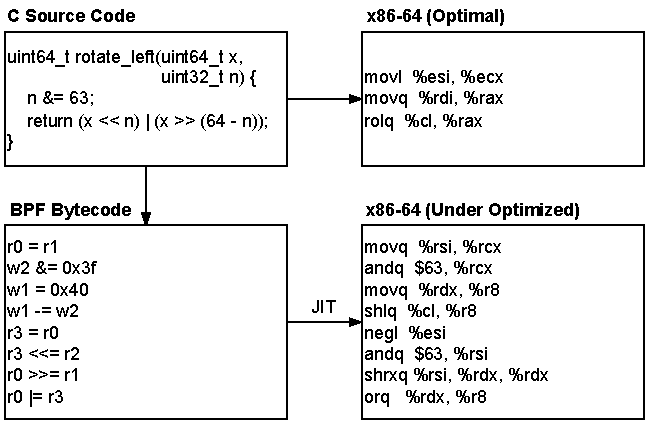
\includegraphics[width=\linewidth]{figures/sec-3-jit-dump.pdf}
  \caption{Compiling a 64-bit rotate through two paths. The direct path compiles C to x86-64 with LLVM, emitting a single \texttt{ROL}. The eBPF path compiles C to eBPF bytecode and then to x86-64 via the eBPF JIT compiler, emitting a longer sequence because the eBPF ISA has no rotate opcode.}
  \label{fig:jit-dump}
\end{figure}


The rotate is not an isolated case. Table~\ref{tab:isa-gap} lists five classes of hardware instructions that have no eBPF opcode equivalent. In each case, the eBPF JIT compiler emits a multi-instruction sequence for an operation the hardware performs in one or two instructions.

\begin{table}[t]
\centering
\small
\caption{Five classes of hardware instructions with no eBPF opcode. Each row gives the number of eBPF instructions needed to emulate the operation and the corresponding native instructions on x86-64 and ARM64.}
\label{tab:isa-gap}
\begin{tabular}{@{}lccc@{}}
\toprule
Capability & \# eBPF insns & x86-64 & ARM64 \\
\midrule
Conditional move & 3 & \texttt{CMOV} & \texttt{CSEL} \\
Rotate & 8 & \texttt{ROL} & \texttt{ROR} \\
Bitfield extract & 8 & \texttt{SHR+AND} & \texttt{UBFX} \\
Endian load & 10 & \texttt{MOVBE} & \texttt{REV+LDR} \\
Wide recompose & 22 & \texttt{MOV} & \texttt{LDR} \\
\bottomrule
\end{tabular}
\end{table}

\subsection{Characterizing the Gap}
\label{subsec:gap}

We characterize the gap with 29 pure-bytecode microbenchmarks covering compute, branch, parser, checksum, string, and packet patterns. Each microbenchmark runs the same source through four execution paths, so each ratio reflects code generation alone. The baseline is the in-kernel eBPF JIT compiler. The three comparison paths are userspace native code, a userspace LLVM-BPF runtime, and an in-kernel native path. We report the median steady-state execution time and exclude load, link, and compile time. Table~\ref{tab:char-micro-artifacts} lists the benchmarks.

\begin{table*}[t]
\centering
\scriptsize
\caption{Authoritative pure-bytecode microbenchmark artifacts used for the eBPF-hardware gap characterization. Artifact suffixes identify the result directories under \texttt{micro/results}. Correctness mismatches count expected-result or retval mismatches across all recorded samples.}
\label{tab:char-micro-artifacts}
\begin{tabular}{@{}llllr@{}}
\toprule
Platform & Suite & Artifact suffix & Runtimes & Mismatches \\
\midrule
x86-64 KVM & Pure bytecode 29 & \texttt{210952\_650695} & kernel, LLVM-BPF, native, kernel native & 0 \\
ARM64 AWS & Pure bytecode 29 & \texttt{063319\_954947} & kernel, LLVM-BPF, native, kernel native & 0 \\
\bottomrule
\end{tabular}
\end{table*}


Most of the gap is in code generation, and the kernel can recover the gap without leaving the kernel. The in-kernel native path keeps the kernel boundary and changes only code generation. On x86-64, the in-kernel native path already runs 1.474$\times$ faster than the eBPF JIT compiler (Table~\ref{tab:char-micro-summary}). The userspace native path runs 1.716$\times$ faster, so leaving the kernel adds only a small speedup beyond changing code generation. The remaining cost lies in the machine code the eBPF JIT compiler generates.

\begin{table*}[t]
\centering
\small
\caption{Pure-bytecode runtime ratios relative to the kernel eBPF JIT. Ratios use median steady-state execution time per benchmark and suite-level geomeans across benchmarks; lower ratio and higher speedup are better.}
\label{tab:char-micro-summary}
\begin{tabular}{@{}lllccc@{}}
\toprule
Platform & Suite & Runtime & Runtime/kernel & Speedup & Wins/losses/ties \\
\midrule
x86-64 KVM & Pure bytecode 29 & Userspace native & 0.583 & 1.716$\times$ & 27/1/1 \\
x86-64 KVM & Pure bytecode 29 & LLVM-BPF userspace & 0.650 & 1.538$\times$ & 27/1/1 \\
x86-64 KVM & Pure bytecode 29 & Kernel native & 0.678 & 1.474$\times$ & 24/2/3 \\
ARM64 AWS & Pure bytecode 29 & Userspace native & 0.467 & 2.141$\times$ & 29/0/0 \\
ARM64 AWS & Pure bytecode 29 & LLVM-BPF userspace & 0.512 & 1.952$\times$ & 29/0/0 \\
ARM64 AWS & Pure bytecode 29 & Kernel native & 0.563 & 1.777$\times$ & 27/0/2 \\
\bottomrule
\end{tabular}
\end{table*}


The gap is systematic and holds across architectures. On x86-64, the in-kernel native path wins 27 of 29 microbenchmarks under a $\pm$2\% tie band (Figure~\ref{fig:char-pure-percase}). On ARM64, the in-kernel native path runs 1.777$\times$ faster than the eBPF JIT compiler and wins 27 of 29 microbenchmarks. The same ordering of paths appears on both architectures (Figure~\ref{fig:char-pure-aggregate}).

\begin{figure}[t]
\centering
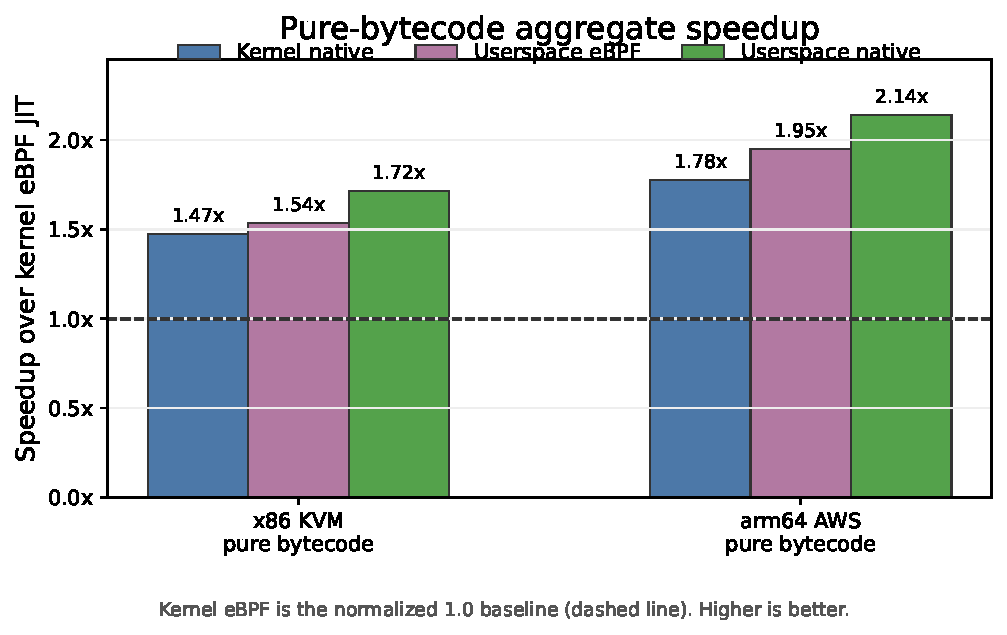
\includegraphics[width=\columnwidth]{figures/sec-3-pure-bytecode-aggregate-20260606.pdf}
\caption{Aggregate pure-bytecode microbenchmark speedup over kernel eBPF JIT. x86 KVM and ARM64 AWS both include kernel native, userspace eBPF, and userspace native. Higher is better; the dashed line is parity.}
\label{fig:char-pure-aggregate}
\end{figure}

\begin{figure*}[t]
\centering
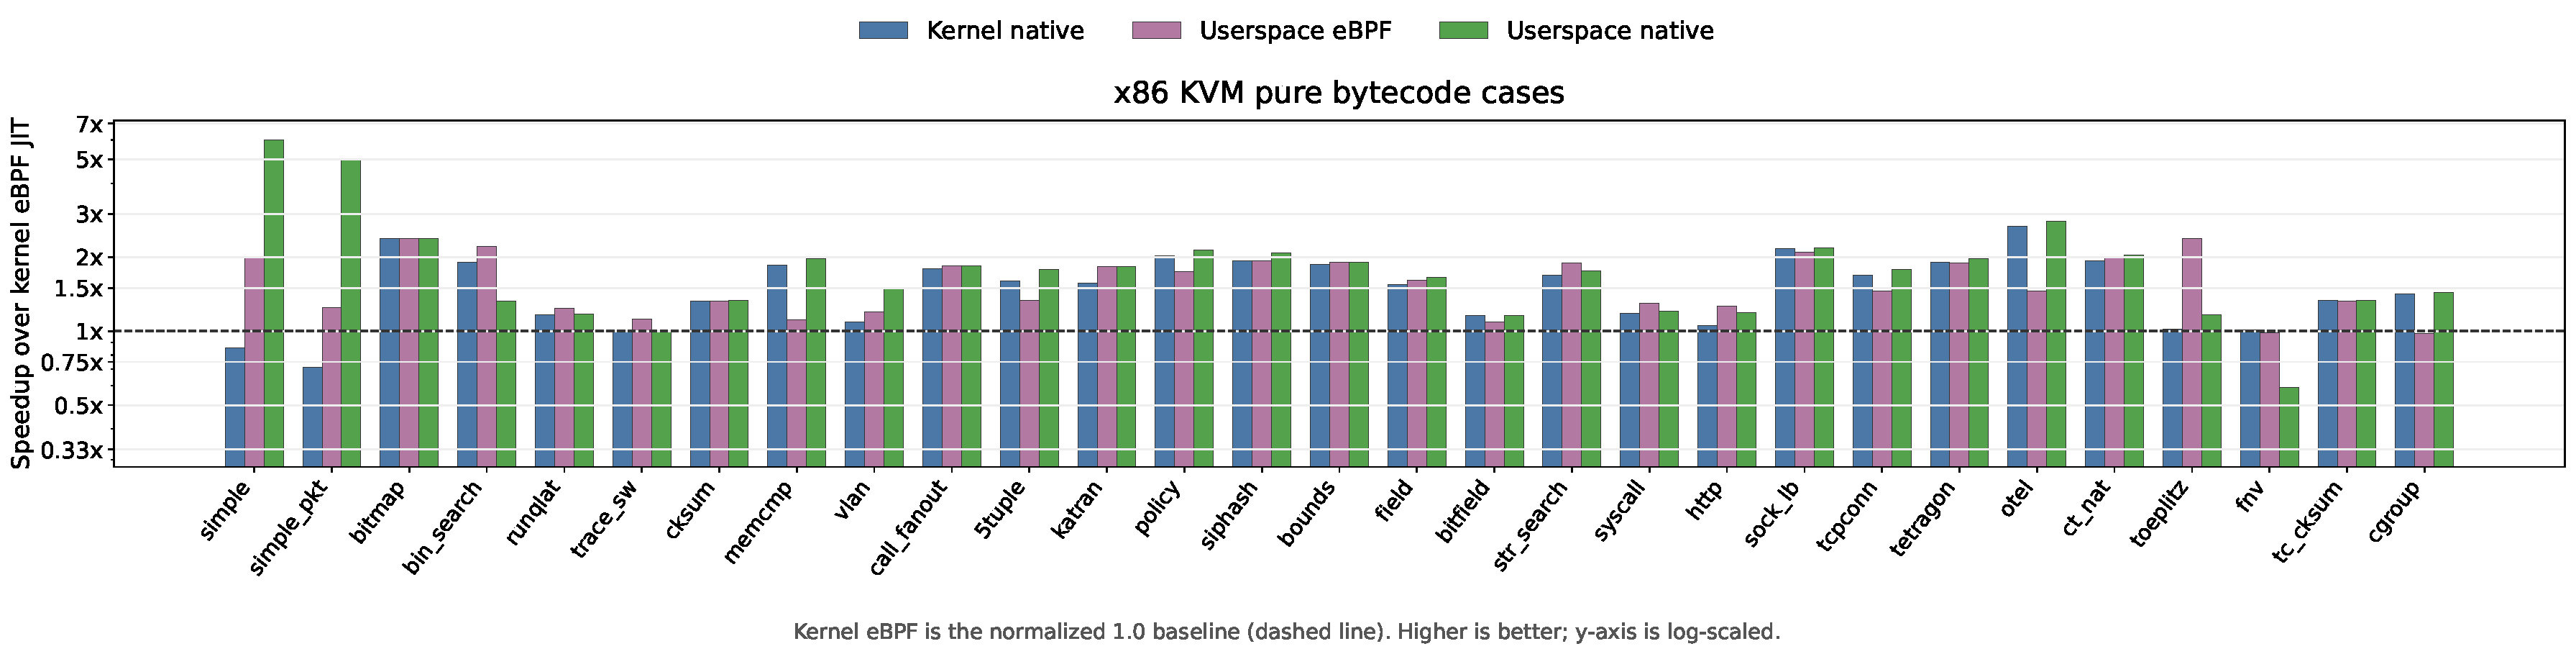
\includegraphics[width=\textwidth]{figures/sec-3-x86-pure-bytecode-percase-20260606.pdf}
\vspace{0.5em}
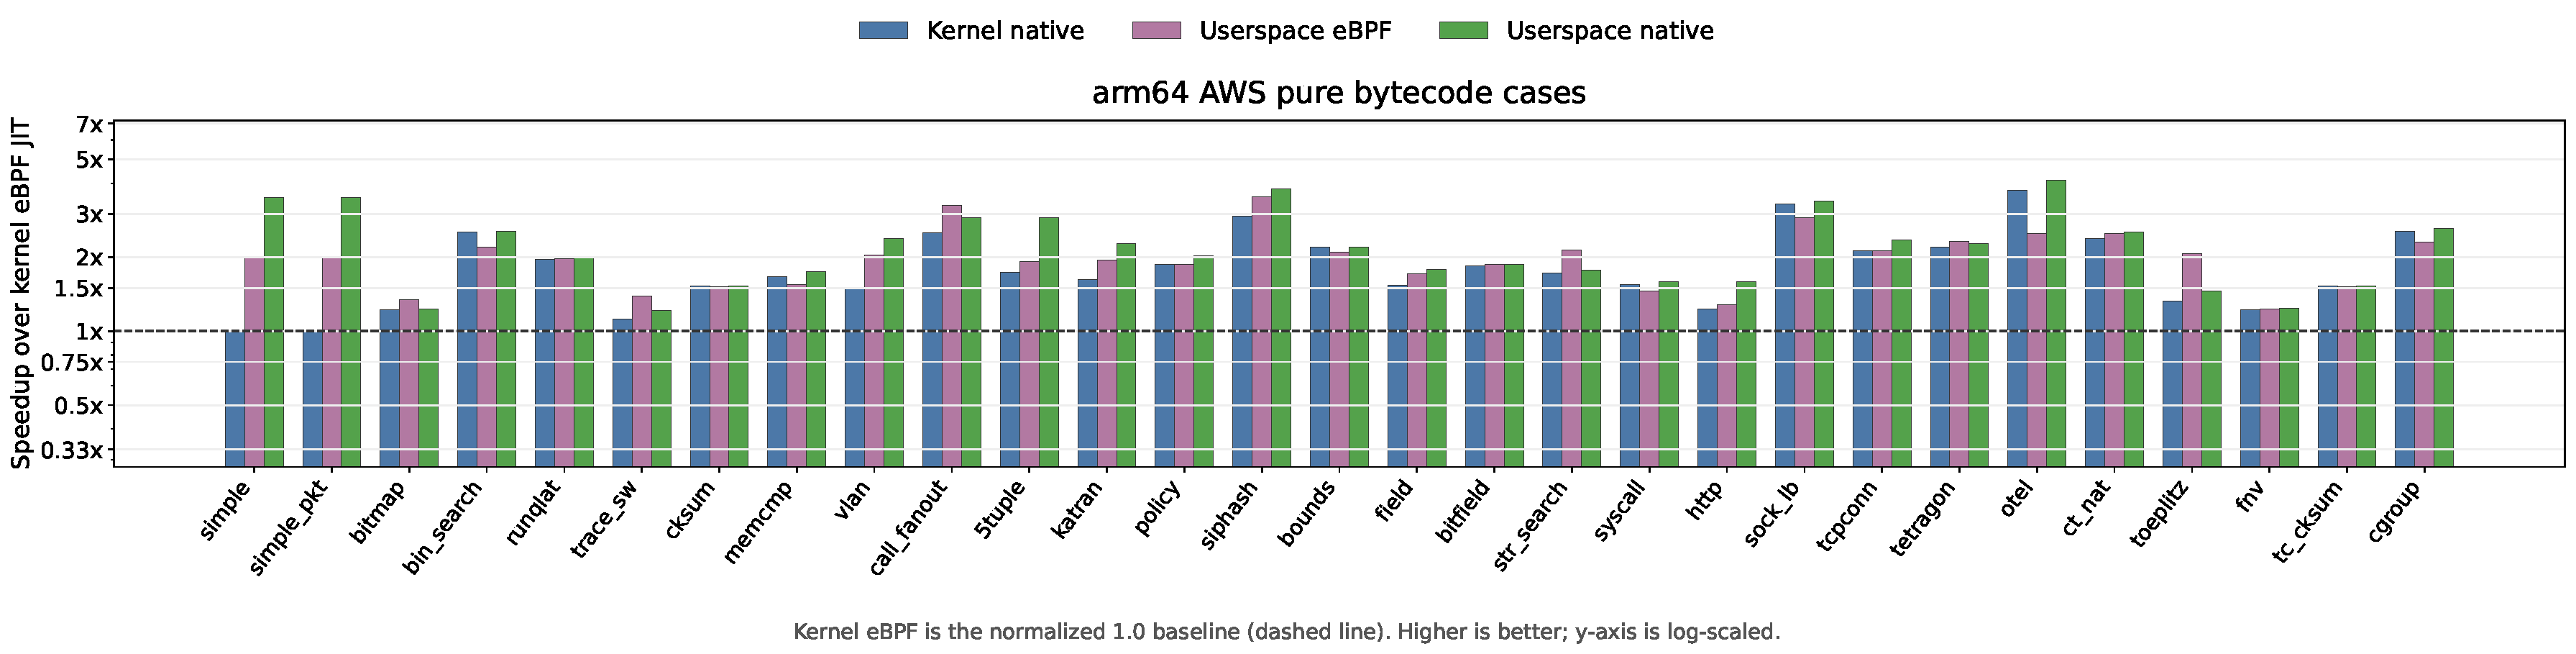
\includegraphics[width=\textwidth]{figures/sec-3-arm64-pure-bytecode-percase-20260606.pdf}
\caption{Per-case pure-bytecode microbenchmark speedup over kernel eBPF JIT. Top: x86 KVM. Bottom: ARM64 AWS. Both platforms report userspace eBPF, userspace native, and kernel native. Higher is better; the dashed line is parity.}
\label{fig:char-pure-percase}
\end{figure*}


The eBPF JIT compiler also emits more machine code than necessary. On x86-64, the in-kernel native path produces machine code 0.541$\times$ the size of the eBPF JIT compiler output. On ARM64, the in-kernel native path produces machine code 0.495$\times$ the size. The decomposed bytecode therefore inflates both runtime and code size.

\subsection{Challenges in Bridging the Gap}
\label{subsec:char-challenges}

Bridging the gap means adding the missing hardware operations to eBPF. Adding an operation to the pipeline faces three challenges, one per stage:

\begin{itemize}
  \item \textbf{Verification:} how to accept a new opcode without adding a transfer function to the verifier, which defines one transfer function per opcode and rejects any unknown opcode (\S\ref{sec:background}).
  \item \textbf{Translation:} how to let the JIT emit native code for an opcode the kernel does not hardcode, given a JIT that dispatches over a fixed opcode set with one case per architecture.
  \item \textbf{Portability:} how to keep execution architecture-specific while keeping verification architecture-independent, since one operation needs different native instructions across architectures (x86-64 \texttt{ROL} vs.\ ARM64 \texttt{ROR}).
\end{itemize}